% Geodesic Equation Visualization
% Demonstrates free fall in curved spacetime as straightest possible path
% Physical interpretation: extremal proper time, freely falling reference frame

\begin{figure}[htbp]
\centering
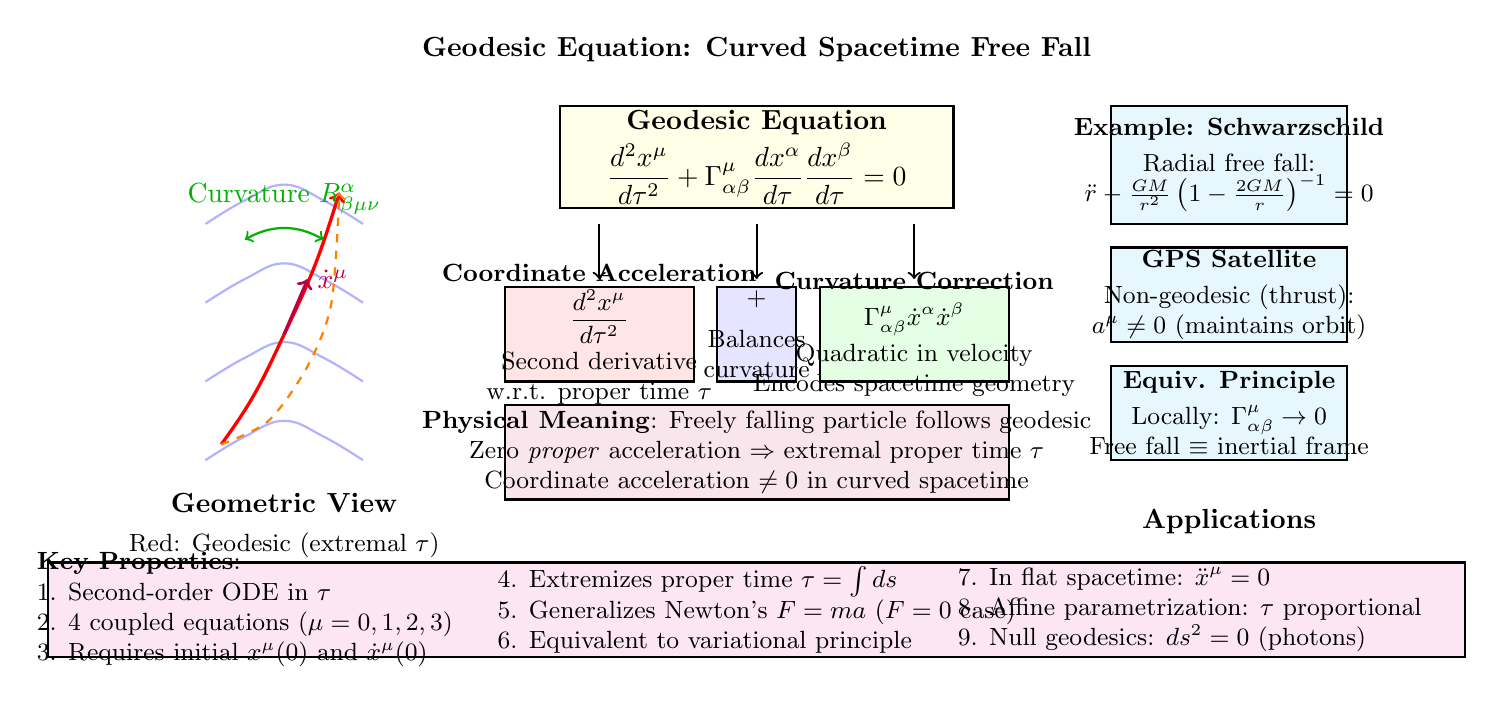
\begin{tikzpicture}[scale=1.0]
    % Title
    \node[anchor=north] at (0,5.5) {\textbf{Geodesic Equation: Curved Spacetime Free Fall}};
    
    % Left side: Curved surface representation
    \begin{scope}[xshift=-6cm]
        % Curved surface grid
        \draw[blue!30, thick] plot[smooth, tension=0.7] coordinates {(-1,0) (-0.5,0.3) (0,0.5) (0.5,0.3) (1,0)};
        \draw[blue!30, thick] plot[smooth, tension=0.7] coordinates {(-1,1) (-0.5,1.3) (0,1.5) (0.5,1.3) (1,1)};
        \draw[blue!30, thick] plot[smooth, tension=0.7] coordinates {(-1,2) (-0.5,2.3) (0,2.5) (0.5,2.3) (1,2)};
        \draw[blue!30, thick] plot[smooth, tension=0.7] coordinates {(-1,3) (-0.5,3.3) (0,3.5) (0.5,3.3) (1,3)};
        
        % Geodesic path (red, thick)
        \draw[red, very thick, ->] plot[smooth, tension=0.7] coordinates {
            (-0.8,0.2) (-0.4,0.8) (0,1.6) (0.4,2.5) (0.7,3.4)
        };
        
        % Alternative non-geodesic path (dashed, orange)
        \draw[orange, thick, dashed, ->] plot[smooth, tension=0.5] coordinates {
            (-0.8,0.2) (-0.2,0.5) (0.3,1.2) (0.6,2.0) (0.7,3.4)
        };
        
        % Tangent vector
        \draw[->, purple, very thick] (0,1.6) -- (0.3,2.3);
        \node[purple, right] at (0.3,2.3) {$\dot{x}^\mu$};
        
        % Curvature annotation
        \draw[<->, green!70!black, thick] (-0.5,2.8) to[bend left=30] (0.5,2.8);
        \node[green!70!black, above] at (0,3.0) {Curvature $R^\alpha_{\beta\mu\nu}$};
        
        \node[below] at (0,-0.3) {\textbf{Geometric View}};
        \node[below, align=center, font=\small] at (0,-0.8) {
            Red: Geodesic (extremal $\tau$)\\
            Orange: Non-geodesic (accelerated)
        };
    \end{scope}
    
    % Center: Equation breakdown
    \begin{scope}
        % Main equation box
        \draw[thick, fill=yellow!10] (-2.5,4.5) rectangle (2.5,3.2);
        \node[align=center] at (0,3.85) {
            \textbf{Geodesic Equation}\\[2pt]
            $\displaystyle \frac{d^2 x^\mu}{d\tau^2} + \Gamma^\mu_{\alpha\beta} \frac{dx^\alpha}{d\tau}\frac{dx^\beta}{d\tau} = 0$
        };
        
        % Component breakdown
        \draw[->, thick] (-2,3.0) -- (-2,2.3);
        \draw[->, thick] (0,3.0) -- (0,2.3);
        \draw[->, thick] (2,3.0) -- (2,2.3);
        
        % Acceleration term
        \draw[thick, fill=red!10] (-3.2,2.2) rectangle (-0.8,1.0);
        \node[align=center, font=\small] at (-2,1.6) {
            \textbf{Coordinate Acceleration}\\[2pt]
            $\displaystyle \frac{d^2 x^\mu}{d\tau^2}$\\[2pt]
            Second derivative\\
            w.r.t. proper time $\tau$
        };
        
        % Connection term
        \draw[thick, fill=blue!10] (-0.5,2.2) rectangle (0.5,1.0);
        \node[align=center, font=\small] at (0,1.6) {
            \textbf{$+$}\\[4pt]
            Balances\\
            curvature
        };
        
        % Christoffel velocity term
        \draw[thick, fill=green!10] (0.8,2.2) rectangle (3.2,1.0);
        \node[align=center, font=\small] at (2,1.6) {
            \textbf{Curvature Correction}\\[2pt]
            $\Gamma^\mu_{\alpha\beta} \dot{x}^\alpha\dot{x}^\beta$\\[2pt]
            Quadratic in velocity\\
            Encodes spacetime geometry
        };
        
        % Physical interpretation
        \draw[thick, fill=purple!10] (-3.2,0.7) rectangle (3.2,-0.5);
        \node[align=center, font=\small] at (0,0.1) {
            \textbf{Physical Meaning}: Freely falling particle follows geodesic\\
            Zero \textit{proper} acceleration $\Rightarrow$ extremal proper time $\tau$\\
            Coordinate acceleration $\neq 0$ in curved spacetime
        };
    \end{scope}
    
    % Right side: Examples
    \begin{scope}[xshift=6cm]
        % Example 1: Schwarzschild
        \draw[thick, fill=cyan!10] (-1.5,4.5) rectangle (1.5,3.0);
        \node[align=center, font=\small] at (0,3.75) {
            \textbf{Example: Schwarzschild}\\[2pt]
            Radial free fall:\\
            $\ddot{r} - \frac{GM}{r^2}\left(1-\frac{2GM}{r}\right)^{-1} = 0$
        };
        
        % Example 2: GPS satellite
        \draw[thick, fill=cyan!10] (-1.5,2.7) rectangle (1.5,1.5);
        \node[align=center, font=\small] at (0,2.1) {
            \textbf{GPS Satellite}\\[2pt]
            Non-geodesic (thrust):\\
            $a^\mu \neq 0$ (maintains orbit)
        };
        
        % Example 3: Equivalence principle
        \draw[thick, fill=cyan!10] (-1.5,1.2) rectangle (1.5,0.0);
        \node[align=center, font=\small] at (0,0.6) {
            \textbf{Equiv. Principle}\\[2pt]
            Locally: $\Gamma^\mu_{\alpha\beta} \to 0$\\
            Free fall $\equiv$ inertial frame
        };
        
        \node[below, align=center] at (0,-0.5) {\textbf{Applications}};
    \end{scope}
    
    % Bottom: Key properties
    \draw[thick, fill=magenta!10] (-9,-1.3) rectangle (9,-2.5);
    \node[align=left, font=\small] at (-6.5,-1.9) {
        \textbf{Key Properties}:\\
        1. Second-order ODE in $\tau$\\
        2. 4 coupled equations ($\mu = 0,1,2,3$)\\
        3. Requires initial $x^\mu(0)$ and $\dot{x}^\mu(0)$
    };
    \node[align=left, font=\small] at (0,-1.9) {
        4. Extremizes proper time $\tau = \int ds$\\
        5. Generalizes Newton's $F = ma$ ($F=0$ case)\\
        6. Equivalent to variational principle
    };
    \node[align=left, font=\small] at (5.5,-1.9) {
        7. In flat spacetime: $\ddot{x}^\mu = 0$\\
        8. Affine parametrization: $\tau$ proportional\\
        9. Null geodesics: $ds^2 = 0$ (photons)
    };
    
\end{tikzpicture}
\caption{Geodesic equation visualization showing free fall as extremal proper time path in curved spacetime. Left: geometric interpretation with geodesic (red) vs non-geodesic (orange) paths. Center: equation component breakdown. Right: physical examples (Schwarzschild, GPS, equivalence principle). Bottom: key mathematical and physical properties.}
\label{fig:geodesic_equation}
\end{figure}
